% -*- mode:latex; mode:flyspell -*-
%% bare_conf.tex
%% V1.3
%% 2007/01/11
%% by Michael Shell
%% See:
%% http://www.michaelshell.org/
%% for current contact information.
%%
%% This is a skeleton file demonstrating the use of IEEEtran.cls
%% (requires IEEEtran.cls version 1.7 or later) with an IEEE conference paper.
%%
%% Support sites:
%% http://www.michaelshell.org/tex/ieeetran/
%% http://www.ctan.org/tex-archive/macros/latex/contrib/IEEEtran/
%% and
%% http://www.ieee.org/

%%*************************************************************************
%% Legal Notice:
%% This code is offered as-is without any warranty either expressed or
%% implied; without even the implied warranty of MERCHANTABILITY or
%% FITNESS FOR A PARTICULAR PURPOSE! 
%% User assumes all risk.
%% In no event shall IEEE or any contributor to this code be liable for
%% any damages or losses, including, but not limited to, incidental,
%% consequential, or any other damages, resulting from the use or misuse
%% of any information contained here.
%%
%% All comments are the opinions of their respective authors and are not
%% necessarily endorsed by the IEEE.
%%
%% This work is distributed under the LaTeX Project Public License (LPPL)
%% ( http://www.latex-project.org/ ) version 1.3, and may be freely used,
%% distributed and modified. A copy of the LPPL, version 1.3, is included
%% in the base LaTeX documentation of all distributions of LaTeX released
%% 2003/12/01 or later.
%% Retain all contribution notices and credits.
%% ** Modified files should be clearly indicated as such, including  **
%% ** renaming them and changing author support contact information. **
%%
%% File list of work: IEEEtran.cls, IEEEtran_HOWTO.pdf, bare_adv.tex,
%%                    bare_conf.tex, bare_jrnl.tex, bare_jrnl_compsoc.tex
%%*************************************************************************

% *** Authors should verify (and, if needed, correct) their LaTeX system  ***
% *** with the testflow diagnostic prior to trusting their LaTeX platform ***
% *** with production work. IEEE's font choices can trigger bugs that do  ***
% *** not appear when using other class files.                            ***
% The testflow support page is at:
% http://www.michaelshell.org/tex/testflow/



% Note that the a4paper option is mainly intended so that authors in
% countries using A4 can easily print to A4 and see how their papers will
% look in print - the typesetting of the document will not typically be
% affected with changes in paper size (but the bottom and side margins will).
% Use the testflow package mentioned above to verify correct handling of
% both paper sizes by the user's LaTeX system.
%
% Also note that the "draftcls" or "draftclsnofoot", not "draft", option
% should be used if it is desired that the figures are to be displayed in
% draft mode.
%
\documentclass[10pt, conference, compsocconf]{IEEEtran}
% Add the compsocconf option for Computer Society conferences.
%
% If IEEEtran.cls has not been installed into the LaTeX system files,
% manually specify the path to it like:
% \documentclass[conference]{../sty/IEEEtran}





% Some very useful LaTeX packages include:
% (uncomment the ones you want to load)

\usepackage{bibspacing}
\setlength{\bibspacing}{\baselineskip}
\usepackage{multirow}
\usepackage{xspace}
\usepackage{bm}
\newcommand{\numtplgynodes}{\ensuremath{|V_r|}\xspace}
\newcommand{\gpunum}{\ensuremath{N_G}\xspace}
\newcommand{\veclenset}{\ensuremath{\bm{V}}\xspace}
\newcommand{\bwset}{\ensuremath{\bm{B}}\xspace}
\newcommand{\mipsset}{\ensuremath{\bm{M}}\xspace}
\newcommand{\corenumset}{\ensuremath{\bm{C}}\xspace}
\newcommand{\expt}{\ensuremath{\bm{E}}\xspace}
\newcommand{\ul}{\underline}
\newcommand{\noname}{The NoNamer\xspace}

% *** MISC UTILITY PACKAGES ***
%
%\usepackage{ifpdf}
% Heiko Oberdiek's ifpdf.sty is very useful if you need conditional
% compilation based on whether the output is pdf or dvi.
% usage:
% \ifpdf
%   % pdf code
% \else
%   % dvi code
% \fi
% The latest version of ifpdf.sty can be obtained from:
% http://www.ctan.org/tex-archive/macros/latex/contrib/oberdiek/
% Also, note that IEEEtran.cls V1.7 and later provides a builtin
% \ifCLASSINFOpdf conditional that works the same way.
% When switching from latex to pdflatex and vice-versa, the compiler may
% have to be run twice to clear warning/error messages.

\addtolength{\floatsep}{-5mm}
% \addtolength{\textfloatsep}{-2mm}
\addtolength{\abovecaptionskip}{-3mm}




% *** CITATION PACKAGES ***
%
%\usepackage{cite}
% cite.sty was written by Donald Arseneau
% V1.6 and later of IEEEtran pre-defines the format of the cite.sty package
% \cite{} output to follow that of IEEE. Loading the cite package will
% result in citation numbers being automatically sorted and properly
% "compressed/ranged". e.g., [1], [9], [2], [7], [5], [6] without using
% cite.sty will become [1], [2], [5]--[7], [9] using cite.sty. cite.sty's
% \cite will automatically add leading space, if needed. Use cite.sty's
% noadjust option (cite.sty V3.8 and later) if you want to turn this off.
% cite.sty is already installed on most LaTeX systems. Be sure and use
% version 4.0 (2003-05-27) and later if using hyperref.sty. cite.sty does
% not currently provide for hyperlinked citations.
% The latest version can be obtained at:
% http://www.ctan.org/tex-archive/macros/latex/contrib/cite/
% The documentation is contained in the cite.sty file itself.






% *** GRAPHICS RELATED PACKAGES ***
%
\ifCLASSINFOpdf
  \usepackage[pdftex]{graphicx}
  \usepackage{color}
  % declare the path(s) where your graphic files are
  % \graphicspath{{../pdf/}{../jpeg/}}
  % and their extensions so you won't have to specify these with
  % every instance of \includegraphics
  % \DeclareGraphicsExtensions{.pdf,.jpeg,.png}
\else
  % or other class option (dvipsone, dvipdf, if not using dvips). graphicx
  % will default to the driver specified in the system graphics.cfg if no
  % driver is specified.
  % \usepackage[dvips]{graphicx}
  % declare the path(s) where your graphic files are
  % \graphicspath{{../eps/}}
  % and their extensions so you won't have to specify these with
  % every instance of \includegraphics
  % \DeclareGraphicsExtensions{.eps}
\fi
% graphicx was written by David Carlisle and Sebastian Rahtz. It is
% required if you want graphics, photos, etc. graphicx.sty is already
% installed on most LaTeX systems. The latest version and documentation can
% be obtained at: 
% http://www.ctan.org/tex-archive/macros/latex/required/graphics/
% Another good source of documentation is "Using Imported Graphics in
% LaTeX2e" by Keith Reckdahl which can be found as epslatex.ps or
% epslatex.pdf at: http://www.ctan.org/tex-archive/info/
%
% latex, and pdflatex in dvi mode, support graphics in encapsulated
% postscript (.eps) format. pdflatex in pdf mode supports graphics
% in .pdf, .jpeg, .png and .mps (metapost) formats. Users should ensure
% that all non-photo figures use a vector format (.eps, .pdf, .mps) and
% not a bitmapped formats (.jpeg, .png). IEEE frowns on bitmapped formats
% which can result in "jaggedy"/blurry rendering of lines and letters as
% well as large increases in file sizes.
%
% You can find documentation about the pdfTeX application at:
% http://www.tug.org/applications/pdftex





% *** MATH PACKAGES ***
%
\usepackage[cmex10]{amsmath}
\usepackage{amssymb}
% A popular package from the American Mathematical Society that provides
% many useful and powerful commands for dealing with mathematics. If using
% it, be sure to load this package with the cmex10 option to ensure that
% only type 1 fonts will utilized at all point sizes. Without this option,
% it is possible that some math symbols, particularly those within
% footnotes, will be rendered in bitmap form which will result in a
% document that can not be IEEE Xplore compliant!
%
% Also, note that the amsmath package sets \interdisplaylinepenalty to 10000
% thus preventing page breaks from occurring within multiline equations. Use:
%\interdisplaylinepenalty=2500
% after loading amsmath to restore such page breaks as IEEEtran.cls normally
% does. amsmath.sty is already installed on most LaTeX systems. The latest
% version and documentation can be obtained at:
% http://www.ctan.org/tex-archive/macros/latex/required/amslatex/math/




\usepackage{algorithm2e}
% *** SPECIALIZED LIST PACKAGES ***
%
% \usepackage{algorithmic}
% \usepackage{program}
% algorithmic.sty was written by Peter Williams and Rogerio Brito.
% This package provides an algorithmic environment fo describing algorithms.
% You can use the algorithmic environment in-text or within a figure
% environment to provide for a floating algorithm. Do NOT use the algorithm
% floating environment provided by algorithm.sty (by the same authors) or
% algorithm2e.sty (by Christophe Fiorio) as IEEE does not use dedicated
% algorithm float types and packages that provide these will not provide
% correct IEEE style captions. The latest version and documentation of
% algorithmic.sty can be obtained at:
% http://www.ctan.org/tex-archive/macros/latex/contrib/algorithms/
% There is also a support site at:
% http://algorithms.berlios.de/index.html
% Also of interest may be the (relatively newer and more customizable)
% algorithmicx.sty package by Szasz Janos:
% http://www.ctan.org/tex-archive/macros/latex/contrib/algorithmicx/




% *** ALIGNMENT PACKAGES ***
%
%\usepackage{array}
% Frank Mittelbach's and David Carlisle's array.sty patches and improves
% the standard LaTeX2e array and tabular environments to provide better
% appearance and additional user controls. As the default LaTeX2e table
% generation code is lacking to the point of almost being broken with
% respect to the quality of the end results, all users are strongly
% advised to use an enhanced (at the very least that provided by array.sty)
% set of table tools. array.sty is already installed on most systems. The
% latest version and documentation can be obtained at:
% http://www.ctan.org/tex-archive/macros/latex/required/tools/


%\usepackage{mdwmath}
%\usepackage{mdwtab}
% Also highly recommended is Mark Wooding's extremely powerful MDW tools,
% especially mdwmath.sty and mdwtab.sty which are used to format equations
% and tables, respectively. The MDWtools set is already installed on most
% LaTeX systems. The lastest version and documentation is available at:
% http://www.ctan.org/tex-archive/macros/latex/contrib/mdwtools/


% IEEEtran contains the IEEEeqnarray family of commands that can be used to
% generate multiline equations as well as matrices, tables, etc., of high
% quality.


%\usepackage{eqparbox}
% Also of notable interest is Scott Pakin's eqparbox package for creating
% (automatically sized) equal width boxes - aka "natural width parboxes".
% Available at:
% http://www.ctan.org/tex-archive/macros/latex/contrib/eqparbox/





% *** SUBFIGURE PACKAGES ***
\usepackage[tight,footnotesize]{subfigure}
% subfigure.sty was written by Steven Douglas Cochran. This package makes it
% easy to put subfigures in your figures. e.g., "Figure 1a and 1b". For IEEE
% work, it is a good idea to load it with the tight package option to reduce
% the amount of white space around the subfigures. subfigure.sty is already
% installed on most LaTeX systems. The latest version and documentation can
% be obtained at:
% http://www.ctan.org/tex-archive/obsolete/macros/latex/contrib/subfigure/
% subfigure.sty has been superceeded by subfig.sty.



%\usepackage[caption=false]{caption}
%\usepackage[font=footnotesize]{subfig}
% subfig.sty, also written by Steven Douglas Cochran, is the modern
% replacement for subfigure.sty. However, subfig.sty requires and
% automatically loads Axel Sommerfeldt's caption.sty which will override
% IEEEtran.cls handling of captions and this will result in nonIEEE style
% figure/table captions. To prevent this problem, be sure and preload
% caption.sty with its "caption=false" package option. This is will preserve
% IEEEtran.cls handing of captions. Version 1.3 (2005/06/28) and later 
% (recommended due to many improvements over 1.2) of subfig.sty supports
% the caption=false option directly:
%\usepackage[caption=false,font=footnotesize]{subfig}
%
% The latest version and documentation can be obtained at:
% http://www.ctan.org/tex-archive/macros/latex/contrib/subfig/
% The latest version and documentation of caption.sty can be obtained at:
% http://www.ctan.org/tex-archive/macros/latex/contrib/caption/




% *** FLOAT PACKAGES ***
%
%\usepackage{fixltx2e}
% fixltx2e, the successor to the earlier fix2col.sty, was written by
% Frank Mittelbach and David Carlisle. This package corrects a few problems
% in the LaTeX2e kernel, the most notable of which is that in current
% LaTeX2e releases, the ordering of single and double column floats is not
% guaranteed to be preserved. Thus, an unpatched LaTeX2e can allow a
% single column figure to be placed prior to an earlier double column
% figure. The latest version and documentation can be found at:
% http://www.ctan.org/tex-archive/macros/latex/base/



%\usepackage{stfloats}
% stfloats.sty was written by Sigitas Tolusis. This package gives LaTeX2e
% the ability to do double column floats at the bottom of the page as well
% as the top. (e.g., "\begin{figure*}[!b]" is not normally possible in
% LaTeX2e). It also provides a command:
%\fnbelowfloat
% to enable the placement of footnotes below bottom floats (the standard
% LaTeX2e kernel puts them above bottom floats). This is an invasive package
% which rewrites many portions of the LaTeX2e float routines. It may not work
% with other packages that modify the LaTeX2e float routines. The latest
% version and documentation can be obtained at:
% http://www.ctan.org/tex-archive/macros/latex/contrib/sttools/
% Documentation is contained in the stfloats.sty comments as well as in the
% presfull.pdf file. Do not use the stfloats baselinefloat ability as IEEE
% does not allow \baselineskip to stretch. Authors submitting work to the
% IEEE should note that IEEE rarely uses double column equations and
% that authors should try to avoid such use. Do not be tempted to use the
% cuted.sty or midfloat.sty packages (also by Sigitas Tolusis) as IEEE does
% not format its papers in such ways.





% *** PDF, URL AND HYPERLINK PACKAGES ***
%
%\usepackage{url}
% url.sty was written by Donald Arseneau. It provides better support for
% handling and breaking URLs. url.sty is already installed on most LaTeX
% systems. The latest version can be obtained at:
% http://www.ctan.org/tex-archive/macros/latex/contrib/misc/
% Read the url.sty source comments for usage information. Basically,
% \url{my_url_here}.





% *** Do not adjust lengths that control margins, column widths, etc. ***
% *** Do not use packages that alter fonts (such as pslatex).         ***
% There should be no need to do such things with IEEEtran.cls V1.6 and later.
% (Unless specifically asked to do so by the journal or conference you plan
% to submit to, of course. )


% correct bad hyphenation here
\hyphenation{op-tical net-works semi-conduc-tor}


\begin{document}
%
% paper title
% can use linebreaks \\ within to get better formatting as desired
\title{An evaluation of space partitioning methods and meta-heuristics based graph partitioning methods for partitioning road network simulations}

% author names and affiliations
% use a multiple column layout for up to two different
% affiliations

\author{\IEEEauthorblockN{Aravind Vasudevan\IEEEauthorrefmark{2},
Quentin Bragard\IEEEauthorrefmark{4},
Anthony Ventresque\IEEEauthorrefmark{4},
David Gregg\IEEEauthorrefmark{2}}
\IEEEauthorblockA{\IEEEauthorrefmark{2}School of Computer Science and Statistics,
Trinity College Dublin, Dublin 2, Ireland\\
Email: vasudeva@scss.tcd.ie, David.Gregg.cs.tcd.ie }
\IEEEauthorblockA{\IEEEauthorrefmark{4}Computer Science Department, University
College Dublin, Ireland\\
Email: Anthony.Ventresque@ucd.ie, quentin.bragard@ucdconnect.ie}}

% conference papers do not typically use \thanks and this command
% is locked out in conference mode. If really needed, such as for
% the acknowledgment of grants, issue a \IEEEoverridecommandlockouts
% after \documentclass

% for over three affiliations, or if they all won't fit within the width
% of the page, use this alternative format:
% 
%\author{\IEEEauthorblockN{Michael Shell\IEEEauthorrefmark{1},
%Homer Simpson\IEEEauthorrefmark{2},
%James Kirk\IEEEauthorrefmark{3}, 
%Montgomery Scott\IEEEauthorrefmark{3} and
%Eldon Tyrell\IEEEauthorrefmark{4}}
%\IEEEauthorblockA{\IEEEauthorrefmark{1}School of Electrical and Computer Engineering\\
%Georgia Institute of Technology,
%Atlanta, Georgia 30332--0250\\ Email: see http://www.michaelshell.org/contact.html}
%\IEEEauthorblockA{\IEEEauthorrefmark{2}Twentieth Century Fox, Springfield, USA\\
%Email: homer@thesimpsons.com}
%\IEEEauthorblockA{\IEEEauthorrefmark{3}Starfleet Academy, San Francisco, California 96678-2391\\
%Telephone: (800) 555--1212, Fax: (888) 555--1212}
%\IEEEauthorblockA{\IEEEauthorrefmark{4}Tyrell Inc., 123 Replicant Street, Los Angeles, California 90210--4321}}




% use for special paper notices
%\IEEEspecialpapernotice{(Invited Paper)}




% make the title area
\maketitle


\begin{abstract}

  Abstract goes here.
  
  % We present a simulated annealing based partitioning technique for
  % heterogeneous applications onto heterogeneous processing
  % architectures. A heterogeneous application is one where tasks differ
  % in the amount of computation and communication that they perform. A
  % heterogeneous architecture on the other hand, is a composition of
  % processing elements that differ in their capabilities to perform
  % computation and communication. Such applications are very common and
  % heterogeneous architectures are becoming more common in today's
  % environment. Task partitioning onto homogeneous architectures to
  % extract parallelism, is a known NP-hard problem.  Heterogeneity
  % greatly complicates the aforementioned partitioning problem. A number
  % of heuristic approaches have been proposed, some using simulated
  % annealing.  The novelty of our approach is two fold: (1) we go a step
  % further than the currently proposed scientific literature, considering
  % heterogeneity at levels of: task parallelism, data parallelism, and
  % communication. (2) We present a novel algorithm that uses simulated
  % annealing to find better partitions in the presence of heterogeneous
  % architectures, data parallel execution units, and significant data
  % communication costs. Our experimental results show that our approach
  % is on orders of magnitudes better compared to standard simulated
  % annealing.


  % gives significantly better results than existing approaches.

  % In this paper we present a simulated annealing based partitioning
  % technique for heterogeneous applications onto heterogeneous processing
  % architectures. A heterogeneous application is one where tasks differ
  % in the amount of computation and communication that they perform. A
  % heterogeneous architecture on the other hand, is a composition of
  % processing elements that differ in their capabilities to perform
  % computation and communication. Such applications are very common and
  % heterogeneous architectures are becoming more common in today's
  % environment. Task partitioning onto homogeneous architectures in-order
  % to extract parallelism, is a known NP-hard problem. Heterogeneity
  % exponentially complicates the aforementioned partitioning problem. A
  % number of heuristic approaches have been proposed for heterogeneous
  % partitioning, some using simulated annealing, to overcome the NP-hard
  % nature of the problem. The novelty of our approach is two fold: (1) we
  % go a step further than the currently proposed scientific literature,
  % considering heterogeneity at levels of: task parallelism, data
  % parallelism, and communication. (2) We quantitatively show an
  % improvement in the simulated annealing algorithm, both in terms of
  % runtime and resulting application latencies, provided the neighbors in
  % the simulated annealing strategy are guided with the temperature
  % rather than being selected randomly as is the established case.


\end{abstract}

\begin{IEEEkeywords}
Graph partitioning, Space partitioning, Simulated Annealing, Genetic Algorithm, Road Network Simlations.

\end{IEEEkeywords}


% For peer review papers, you can put extra information on the cover
% page as needed:
% \ifCLASSOPTIONpeerreview
% \begin{center} \bfseries EDICS Category: 3-BBND \end{center}
% \fi
%
% For peerreview papers, this IEEEtran command inserts a page break and
% creates the second title. It will be ignored for other modes.
\IEEEpeerreviewmaketitle



\section{Introduction}

Introduction goes here.

Our \textbf{key contributions} in this paper are:

\begin{itemize}
\item 
\item 
\item 
\item 
\end{itemize}

The rest of the paper is arranged as
follows. 

\section{Related Work}
\label{sec:related-work}

\section{FORMALIZATION OF THE PROBLEM STATEMENT}
\label{sec:form}

In this paper we conduct a comparison of different methods of partitioning a road network graph based on some metrics. This section defines what a road network graph is and presents the formal definition of the metrics.

\subsection{The Road Network Graph}
\label{sec:form-road-netw-grap}
The road network of a city can be represented by a directed cyclic graph~\cite{holden1995mathematical} $G(V, E)$ where $V$ denotes the vertex set and $E$ denotes the edge set. Every edge $e_{ij} \in E$ in the graph represents a unidirectional road in the city that connects intersection $v_i$ to intersection $v_j$. Every vertex $v_i \in V$ denotes an intersection of two or more roads. A weight $w_{ij}$ is associated with the edge $e_{ij}$ that is representative of the traffic that flows through that road. As discussed in Section~\ref{sec:futu}, we intend to increase the number of weights that can be associated with every edge to be able to represent the number of lanes, length of the road, importance of the road etc. as part of our future work.

\subsection{Partitioning a graph}
\label{sec:form-part}
For the sake of completeness of the graph definition, we also assign weights to the vertices denoted by $W_i$, which is defined as follows :
\begin{equation}
\label{eq:vertex-weight}
W_i = \sum\limits_{\forall j \in neighbours(i)} w_{ij}
\end{equation}

\noindent where $neighbours(i)$ is the set of all nodes in $V$ that receive an outgoing edge from $v_i$. 

The problem of partitioning a graph has a 2 dimensional space, where one axis represents the node ID(representing the intersection) and the other represents the partition ID. Each point in this 2-D space represents an \textit{\{intersection,partition\}} pair which implies this intersection is mapped onto this partition. We define a ``state'' to be a collection of $|V|$ points such that each intersection is mapped to exactly one partition. The total number of possible ``states'' in this discrete space is $|V|^{p}$, where $p$ is the number of required partitions.

\subsection{Formalizing the objective function}
\label{sec:form-obje-func}

To effectively perform a distributed road network simulation, one must fully understand the effects of dividing the workload(the road network graph to be simulated) into the required number of partitions. To this end, we define three heuristics\{cite papers\} that are widely accepted in the community, to measure the effectiveness of a ``partitioning scheme''. 

We define a partitioning scheme on the given road network $G$, $\lambda_G \in \Lambda_G$(where $\Lambda_G$ is the set of all possible partitioning schemes of the given graph $G$ onto $p$ partitions) as a function that maps every node $v_i$ from the road network graph to a partition. Please note that we will use the terms ``node'', ``vertex'' and ``intersection'' interchangeably.
\begin{equation}
\label{eq:part-sche}
\lambda_G(v_i) \in \{P_0,\dots,P_{p-1}\}, \forall v_i \in V
\end{equation}

\noindent where $P_i$ denotes the $i^{th}$ partition. For the following discussion we denote the weight of the $i^{th}$ partition($P_i$) as $w(P_i)$. One of the primary objectives of road network partitioning for distributed simulation is to minimize the execution time of the simulation time. To this end, we aim to minimize the weight of the \textbf{heaviest partition($\lambda_G^{max}$)} as described by the following equation,

\begin{equation}
\label{eq:metric1}
\lambda_G^{max} = max(w(P_i)), \forall P_i \in \{P_0,\dots,P_{p-1}\}
\end{equation}

\noindent The execution time of a distributed simulation also depends on the amount of \textbf{inter-partition communication}($\lambda_G^{comm}$). In order to reduce this inter-partition communication, we minimize the following metric,

\begin{equation}
\label{eq:metric2}
\lambda_G^{comm} = \sum\limits_{i \in \{v_0,\dots,v_{|V|-1}\}}{\sum\limits_{j \in \{v_0,\dots,v_{|V|-1}\}}{w(e_{ij})}} , s.t. \lambda_G(i) \neq \lambda_G(j)
\end{equation}

\noindent The final metric that we consider is the \textbf{evenness}($\lambda_G^\sigma$) of the partitions. In a scenario in which the underlying architecture consists of homogeneous execution units(i.e. a vertex of the road network graph takes equally long to simulate on any machine in the underlying architecture) and where communication plays a less significant role(i.e. powerful communication backbone), this metric plays a very important role as it defines how varied each machine is loaded.

\begin{equation}
\label{eq:metric3-mean}
\lambda_G^\mu = \frac{\sum\limits_{P_i \in \{P_0,\dots,P_{p-1}\}} w(P_i)}{p}
\end{equation}

\begin{equation}
\label{eq:metric3}
\lambda_G^\sigma = \frac{\sqrt{\sum\limits_{P_i \in \{P_0,\dots,P_{p-1}\}} (w(P_i) - \lambda_G^\mu)^2}}{p}
\end{equation}

\noindent The importance of these metrics vary hugely depending on the underlying architecture onto which these partitions are mapped onto and hence we present the metrics without probing into their relative importance. In the next section, we present an overview of the methods that are compared under the purview of road network partitioning.

%\section{Generating the task graph}
\label{sec:gener-task-graph}

The compilation tool-chain is described in Figure~\ref{fig:5a}. Our
framework can be used in conjunction with the polyhedral model and other
compiler frameworks described in~\cite{atiw09,ubon08}.  Our framework
takes as input the output from these tuning frameworks, built for single
processing element systems and expands it to a multi-core heterogeneous
architecture.

\begin{figure*}[t!]
  \centering
  \subfigure[The compilation tool-chain]{
    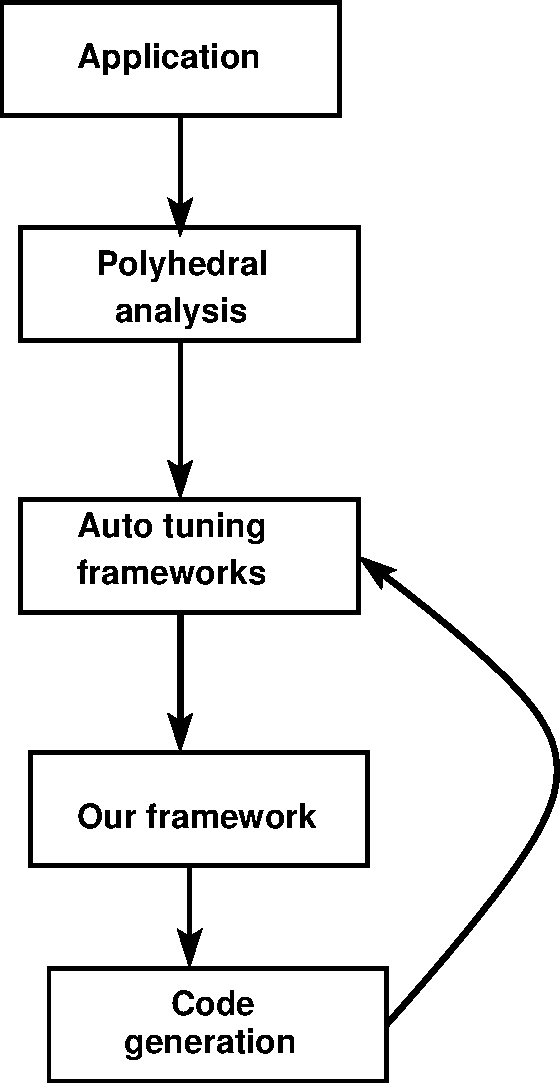
\includegraphics[scale=0.3]{./figures/tool_chain}
    \label{fig:5a}
  }
  \subfigure[The task graph for the Jacobi example]{
    \scalebox{0.4}{\input{./figures/jacobi.pdf_t}}
    % 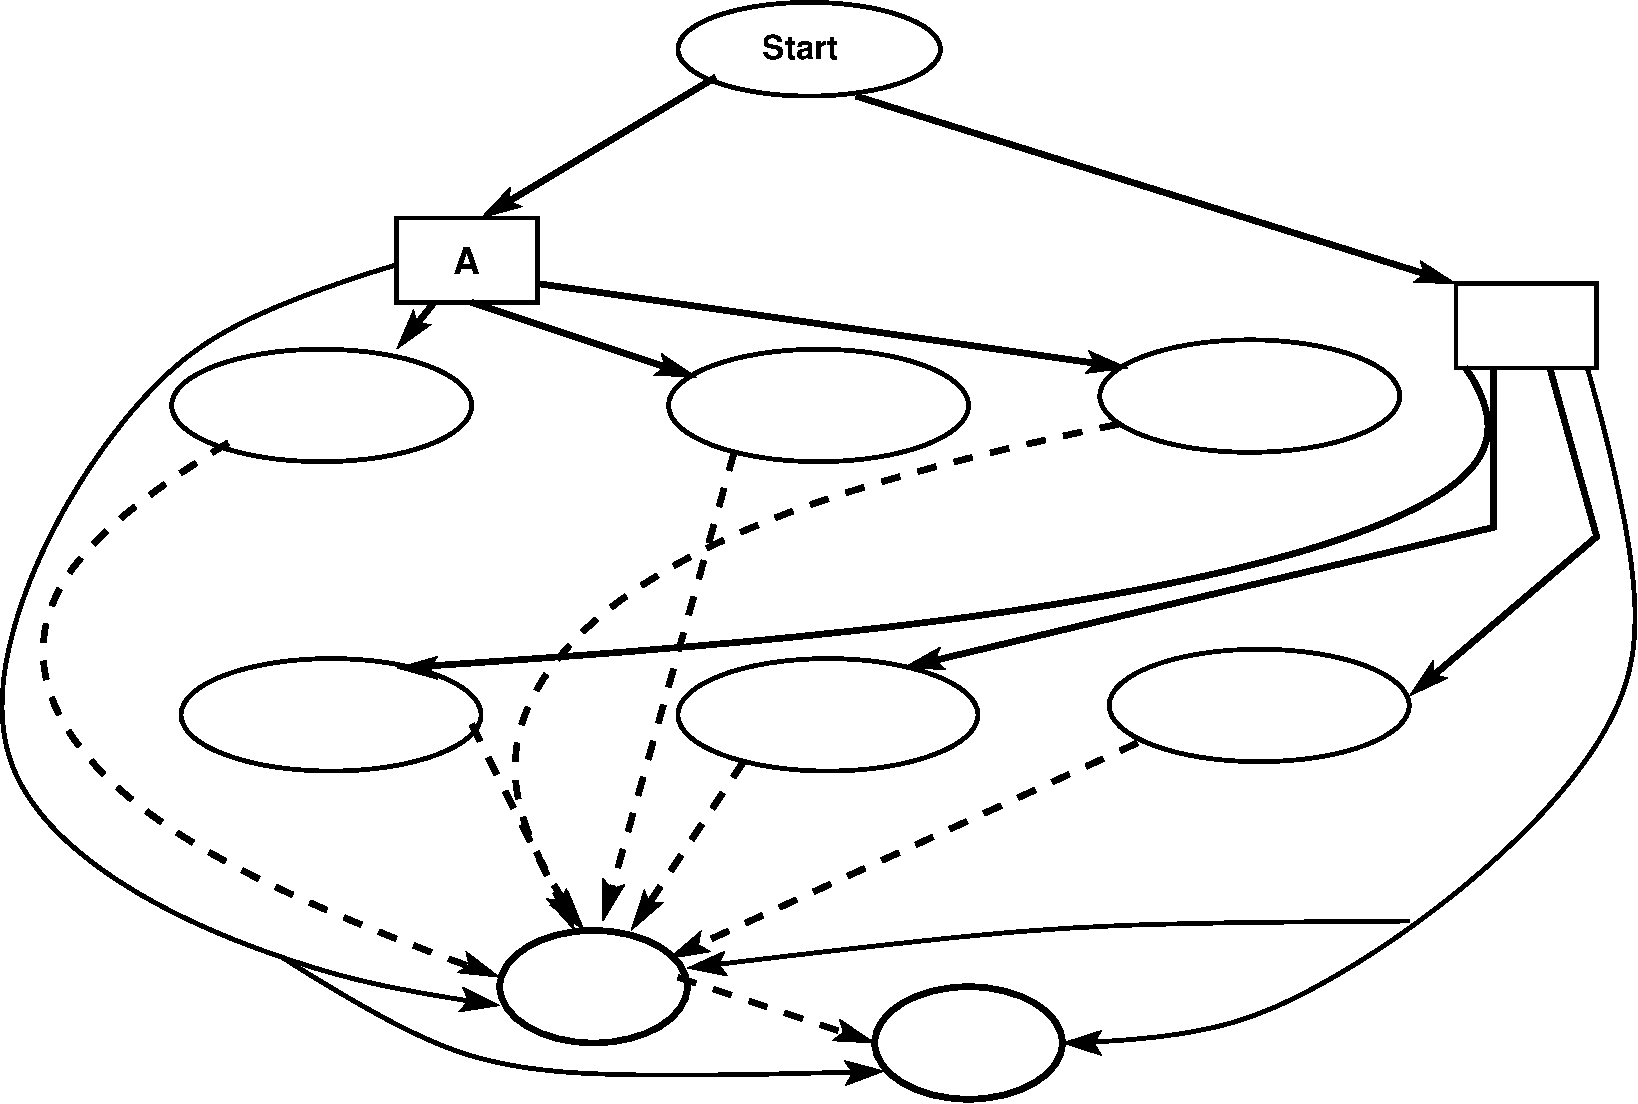
\includegraphics[scale=0.4]{./figures/jacobi}
    \label{fig:5b}
  }
  \caption{Compilation tool-chain and an example task graph}
  \label{fig:5}
\end{figure*}

In this section we use the very popular Jacobi~\cite{jacobi2} stencil
computation to describe how our framework extracts a task graph from the
application for partitioning onto the underlying architecture. Jacobi is
an important stencil computation used in a plethora of domains such as
fluid dynamic and hence, it is worth investigating performance
improvements for Jacobi.

In Figure~\ref{fig:4}, statements S1 and S2 initialize 2D Jacobi
matrices. Next, the actual stencil computation is carried out in
statement S3, for \texttt{TSTEPS} iterations. Finally, statement S4,
transfers the calculated data from matrix \texttt{B} to \texttt{A}.

\begin{scriptsize}
  \begin{figure}[h!]
    \centering
    \small{
\begin{verbatim}
 //Task and data-parallel
 for (int i=0;i<M; ++i){
  for (int j=0;j<N; ++j){
   S1: A[i][j] = (i*j+4.0/N)
   S2: B[i][j] = (i*j+9.0/N)
  }
 }
 for (int k=0;k<TSTEPS;++k){
  for (int i=1; i<M-1; ++i)
   for (int j=1; j<N-1; ++j)
    S3: B[i][j] = 0.2*(A[i][j]+A[i][j-1]
              +A[i][j+1]+A[i-1][j])

  //Data-parallel
  for (int i=1; i<M; ++i)
   for (int j=1; j<N; ++j)
    S4: A[i][j] = B[i][j]
 }
\end{verbatim}
    }
    \caption{Example 2-dimensional Jacobi stencil computation}
    \label{fig:4}
  \end{figure}
\end{scriptsize}

The task graph for the 2D Jacobi stencil computation is shown in
Figure~\ref{fig:5b}. The initialization phase of the Jacobi example
consist of both task and data parallelism. In Figure~\ref{fig:5b}, the
first and second row of statements $S1_1$ to $S1_m$ and $S2_1$ to
$S2_m$, show various loop tiles that are generated for execution onto
different processors for statements S1 and S2, respectively. Each of
these nodes indicate vector computations. Sample vector code within any
one of these assignment nodes when assigned to an Intel SSE3 unit is
shown in Figure~\ref{fig:6}. Similar vector code is generated in the ptx
format for GPU allocations. We keep a count of the number of
instructions for each of these nodes. There are two counts: (1) the
number of instructions a node needs to execute iteratively. For example,
node S3 (representing statement S3 in the Jacobi example) needs to
iterate 998001000 times for a 1000 $\times$ 1000 matrix with
\texttt{TSTEPS} itself set to a 1000, provided it is not vectorized as
shown in Figure~\ref{fig:5b}. (2) Nodes $S1_1$ to $S1_m$ and $S2_1$ to
$S2_m$ only need to be executed once, but have a large vector count.

Each ellipse in the task-graph is connected to a store. Stores are
represented as boxes in the task-graph. Stores have their instruction
count and vector length count set to 0. Every statement depending upon
its vector length requires different amount of data to carry out the
computation. This data needs to be transferred from the store (the main
memory in most cases) to the caches where the task nodes are going to be
executed. We represent the amount of data to be transferred in the
task-graph in bits. For example, node $S1_1$ with a smaller vector
length of 16, requires 2.2KB of data to be transferred to its cache for
computation. Node S3 on the other hand, being non-vectorized requires
15KB of data to be transferred to its cache.

Finally, the task graph also consists of dependence edges. In
Figure~\ref{fig:5b}, the dependence edges are marked with the dashed
lines. Dependence edges, as the name suggests show the dependence
between statements in the application. For example, statements S1 and S2
are independent of each other. But, statements S3 and S4 are dependent
upon these aforementioned statements. Dependence edges do not have any
weights. Once partitioned, the task-graph can then be scheduled
statically or dynamically (work stealing~\cite{rblu99}, say) using these
dependence edges.

\begin{figure}[h!]
  \centering
  \small{
\begin{verbatim}
LCPI0_0:
 .long	1018444121 ## float 2.200000e-02
 .long	1021128475 ## float 2.700000e-02
 .long	1023611503 ## float 3.200000e-02
 .long	1024953680 ## float 3.700000e-02

 movaps	LCPI0_0(%rip), %xmm8
\end{verbatim}
  }
  \caption{Example vector code running on the Intel SSE unit}
  \label{fig:6}
\end{figure}




%%% Local Variables: 
%%% mode: latex
%%% TeX-master: "bare_conf"
%%% End: 


%\section{Generating the resource graph}
\label{sec:gener-reso-graph}


\begin{figure}[t!]
  \centering
  % \includegraphics[scale=0.42]{./figures/jacobi2d}
  \scalebox{0.38}{\section{Generating the resource graph}
\label{sec:gener-reso-graph}


\begin{figure}[t!]
  \centering
  % \includegraphics[scale=0.42]{./figures/jacobi2d}
  \scalebox{0.38}{\section{Generating the resource graph}
\label{sec:gener-reso-graph}


\begin{figure}[t!]
  \centering
  % \includegraphics[scale=0.42]{./figures/jacobi2d}
  \scalebox{0.38}{\input{./figures/resource_graph.pdf_t}}
  \caption{An example resource graph}
  \label{fig:1r}
\end{figure}

We use synthetically generated graphs to test our framework, because in
a heterogeneous setup, we do not know the exact nature of the processing
elements being utilized. For example, a setup might consist of a Tesla
Nvidia GPU core connected to an Atmel micro-processor. It is also
possible that a CELL processing unit is connected to a X86 processing
element. Moreover, we cannot judge beforehand the type of bus
connections one might have on this multi-core system. In order to
overcome these issues we take a more statical view of the process. We
use synthetically generated topologies to test our framework. One such
synthetically generated resource graph is shown in Figure~\ref{fig:1r}.

In the resource graph in Figure~\ref{fig:1r}, the processing elements
are denoted via boxes. Each processing element consists of two
decorations following the previously defined formalism in
Section~\ref{sec:form-reso-graph}. In Figure~\ref{fig:1r} the processing
elements are labeled from \texttt{A} through to \texttt{P} and are
placed in a 2D tiled topology. For processing element \texttt{A} the
MIPS count is provided as $W^A_0$, while the vector length count is
provided as $W^A_1$. The bandwidth connecting the various processing
elements are denoted via $W^c$.

%%% Local Variables: 
%%% mode: latex
%%% TeX-master: "bare_conf"
%%% End: 
}
  \caption{An example resource graph}
  \label{fig:1r}
\end{figure}

We use synthetically generated graphs to test our framework, because in
a heterogeneous setup, we do not know the exact nature of the processing
elements being utilized. For example, a setup might consist of a Tesla
Nvidia GPU core connected to an Atmel micro-processor. It is also
possible that a CELL processing unit is connected to a X86 processing
element. Moreover, we cannot judge beforehand the type of bus
connections one might have on this multi-core system. In order to
overcome these issues we take a more statical view of the process. We
use synthetically generated topologies to test our framework. One such
synthetically generated resource graph is shown in Figure~\ref{fig:1r}.

In the resource graph in Figure~\ref{fig:1r}, the processing elements
are denoted via boxes. Each processing element consists of two
decorations following the previously defined formalism in
Section~\ref{sec:form-reso-graph}. In Figure~\ref{fig:1r} the processing
elements are labeled from \texttt{A} through to \texttt{P} and are
placed in a 2D tiled topology. For processing element \texttt{A} the
MIPS count is provided as $W^A_0$, while the vector length count is
provided as $W^A_1$. The bandwidth connecting the various processing
elements are denoted via $W^c$.

%%% Local Variables: 
%%% mode: latex
%%% TeX-master: "bare_conf"
%%% End: 
}
  \caption{An example resource graph}
  \label{fig:1r}
\end{figure}

We use synthetically generated graphs to test our framework, because in
a heterogeneous setup, we do not know the exact nature of the processing
elements being utilized. For example, a setup might consist of a Tesla
Nvidia GPU core connected to an Atmel micro-processor. It is also
possible that a CELL processing unit is connected to a X86 processing
element. Moreover, we cannot judge beforehand the type of bus
connections one might have on this multi-core system. In order to
overcome these issues we take a more statical view of the process. We
use synthetically generated topologies to test our framework. One such
synthetically generated resource graph is shown in Figure~\ref{fig:1r}.

In the resource graph in Figure~\ref{fig:1r}, the processing elements
are denoted via boxes. Each processing element consists of two
decorations following the previously defined formalism in
Section~\ref{sec:form-reso-graph}. In Figure~\ref{fig:1r} the processing
elements are labeled from \texttt{A} through to \texttt{P} and are
placed in a 2D tiled topology. For processing element \texttt{A} the
MIPS count is provided as $W^A_0$, while the vector length count is
provided as $W^A_1$. The bandwidth connecting the various processing
elements are denoted via $W^c$.

%%% Local Variables: 
%%% mode: latex
%%% TeX-master: "bare_conf"
%%% End: 


%\section{Simulated annealing}
\label{sec:simulated-annealing}

Simulated Annealing~\cite{skir83} is a generic probabilistic algorithm
for finding the global optimum of a given function,
$\mathcal{F}: \mathbb{R} \rightarrow \mathbb{R}$, which has a large
search space.  Simulated Annealing in most of the cases is cheaper than
exhaustive enumeration, which is exhaustively listing the entire search
space. Since it is a Monte Carlo method it will always terminate and the
solution need not be the most optimal but in general considered to be a
good approximation of the optimum.

% \subsection{Overview}

% <<<<<<< HEAD
% In general SA is a non-greedy heuristic algorithm which explores the
% search space by moving from a higher temperature to a lower
% temperature. The algorithm always accepts moves to a better solution,
% determined by evaluating an \emph{objective function} and sometimes
% accpets moves to worse states with a probability that changes with
% temperatures. Initially, when the temperature is high, the algorithm is
% more tolerable and accepts moves to worse states with a higher
% probability. As the temperature falls down, this probability decreases
% and the alogrithm is less tolerant towards solutions with a worse value
% for the objective function.

% This is the reason why SA is not a purely greedy algorithm as it accepts
% moves to bad states with some probability which enables it to move out
% of local maximas\/minimas. But the algorithm becomes more greedier as
% the temperature decreases. Figure~\ref{fig:temperature_drop} shows how
% the temperature drops and how this acceptance probability changes with
% this drop in temperature.

% \subsection{From the mapping problem standpoint}

% \begin{algorithm}
%   \DontPrintSemicolon
%   \KwIn{Initial Mapping $\zeta_0$ and Starting Temperature $T_0$}
%   \KwOut{Best Mapping $\zeta_{best}$}
%     $\zeta \leftarrow \zeta_0$\;
%     $C \leftarrow OBJECTIVE\_FUNCTION(\zeta_0)$\;
%     $\zeta_{best} \leftarrow \zeta$\;
%     $C_{best} \leftarrow C$\;
%     \Return $\zeta_{best}$
%   \caption{$Simulated\_Annealing(\zeta_0, T_0)$}
%   \label{algo:SA}
% \end{algorithm}

% Figure~\ref{algo:SA} represents the pseudocode for our algorithm. We
% begin by choosing some initial starting point for our state space
% exploration, which from the mapping problem standpoint is some initial
% mapping of tasks from $V_t$ to PEs $V_r$. We choose our initial mapping
% to be all tasks from $V_t$ mapped onto some random PE $j \in V_r$. This
% is a good idea because we have observed that this puts tightly coupled
% tasks, i.e. tasks that communicate heavily, on the same PE since moving
% them onto different PEs would incur more costs and would thus lead to a
% bad state.
% =======
SA is a heuristic algorithm which explores the search
space by moving from a higher temperature to a lower temperature. The algorithm
always accepts moves to a better solution, determined by evaluating an
\textit{objective function} and sometimes accepts moves to worse states with a
probability that changes with temperature. Initially, when the temperature is
high, the algorithm is more tolerable and accepts moves to worse states with a
higher probability. As the temperature falls down, this probability decreases
and the algorithm is less tolerant towards solutions with a worse value for the
objective function.

This is the reason why SA is not a purely greedy algorithm as it accepts
moves to bad states with some probability which enables it to move out
of local maxima and minima. However, the algorithm becomes greedier as
the temperature decreases. Figure~\ref{fig:7} shows how the temperature
drops for different values of a annealing parameter $q$ which is
described in Sections~\ref{sec:conventional-SA}
and~\ref{sec:our-improved-sa}.

\subsection{Conventional Simulated Annealing : From the mapping problem
  standpoint}
\label{sec:conventional-SA}

\begin{algorithm}[h!]
  \small{
    \caption{$Simulated\_Annealing(\zeta_0, \mathcal{T}_0)$}
    \label{algo:SA}
    % \DontPrintSemicolon
    \KwIn{Initial Mapping $\zeta_0$ and Starting and Final Temperatures
$\mathcal{T}_0$, $\mathcal{T}_f$}
    \KwOut{Best Mapping $\zeta_{best}$}
    $\zeta_{current} \leftarrow \zeta_0$ \;
    $C_{current} \leftarrow OBJECTIVE\_FUNCTION(\zeta_0)$ \;
    $\zeta_{best} \leftarrow \zeta_{current}$\;
    $C_{best} \leftarrow C_{current}$\;
    $R \leftarrow 0$\;
    \For {$i \leftarrow 0\ to\ \infty$}{
      $\mathcal{T}_{current} \leftarrow NEXT\_TEMPERATURE(\mathcal{T_0,i})$\;
      $\zeta_{new} \leftarrow NEXT\_STATE(\zeta_{current}, \mathcal{T})$\;
      $C_{new} \leftarrow OBJECTIVE\_FUNCTION(\zeta_{new})$\;
      $\Delta C \leftarrow C_{new} - C_{current}$\;
      $r \leftarrow RAND()$\;
      $p \leftarrow ACCEPTANCE\_PROBABILITY(\Delta C, \mathcal{T}_{current})$\;
      \If{$\Delta C \textless 0$ or $r \textless p$}{
        \If{$C_{new} \textless C_{best}$}{
          $\zeta_{best} \leftarrow \zeta_{new}$\;
          $C_{best} \leftarrow C_{new}$\;
          $\zeta_{current} \leftarrow \zeta_{new}$\;
          $C_{current} \leftarrow C_{new}$\;
          $R \leftarrow 0$\;
        }
      }
      \Else{
        \If{$\mathcal{T}_{current} \leq \mathcal{T}_f$}{
          $R \leftarrow R+1$\;
          \If{$R \geq R_{max}$}{break}
        }
      }
    }
    \Return $\zeta_{best}$
  }
\end{algorithm}

Algorithm~\ref{algo:SA} represents the pseudo-code for the novel
algorithm presented by ~\cite{hors06} which maps applications onto
Multiprocessor SoCs.  The \textit{OBJECTIVE\_FUNCTION} evaluates
execution time of a specific mapping by calling the
scheduler. $\zeta_0,\ \zeta_{current}$ and $\mathcal{T}_0,\
\mathcal{T}_{current}$ are the initial and current mapping and
temperatures, respectively. The \textit{NEXT\_STATE} function moves a
random task to a random PE different than the original
PE. \textit{NEXT\_TEMPERATURE} is chosen so that the annealing schedule
is proportional to the number of tasks and resources and is given by,

\begin{equation}
\label{eq:3}
\textit{NEXT\_TEMPERATURE}(\mathcal{T}_0, i) = \mathcal{T}_0*q^{\lfloor
\frac{i}{L} \rfloor}
\end{equation}
\noindent
where q is the proportion of temperature preserved in each temperature
level. % In their paper, q was set as $0.95$ and
L is the number of iterations in one temperature level. Multiple
iterations are achieved at a single temperature level by using the
\texttt{floor} function, since $\lfloor \frac{i}{L} \rfloor$ moves to a
new value only at every integral multiple of $L$.

\begin{equation}
L = |V_t|*(|V_r| - 1)
\end{equation}

The \textit{ACCEPTANCE\_PROBABILITY} function is modified from its
traditional form: $\frac{1}{1+exp(\frac{\Delta C}{\mathcal{T}})}$ to
adapt automatically to different cost function value ranges and graphs
with different task execution times. This is done by normalizing the
change in cost, $\Delta C$,

\begin{equation}
  \begin{array}{c}
    ACCEPTANCE\_PROBABILITY(\Delta C, \mathcal{T}) \\ 
    = \frac{1}{1+exp(\frac{\Delta C}{0.5C_0\mathcal{T}})}
  \end{array}
\end{equation}

The initial temperature $\mathcal{T}_0$ of the annealing schedule is
selected as:

\begin{equation}
\mathcal{T}_0 = \frac{t_{max}}{t_{minsum}}
\end{equation}
\noindent
where $t_{max}$ is the maximum execution time for any task $i \in V_t$
on any PE $j \in V_r$ and $t_{minsum}$ is the sum of execution time of
all tasks in $V_t$ on the fastest PE $j_{fastest} \in V_r$.

The final temperature of the annealing schedule is selected as:

\begin{equation}
\mathcal{T}_f = \frac{t_{min}}{t_{maxsum}}
\end{equation}
\noindent
where $t_{min}$ is the minimum execution time for any task $i \in V_t$
on any PE $j \in V_r$ and $t_{maxsum}$ is the sum of execution time of
all tasks in $V_t$ on the slowest PE $j_{slowest} \in
V_r$. % In both the
% cases, $k$ is a constant and $k=1$ is suitable for all our experiments.

\subsection{Our Improved SA Approach}
\label{sec:our-improved-sa}

We made novel changes to the aforementioned algorithm and associated
heuristics as prescribed by Orsilla et al~\cite{hors06}. The reasons
behind these changes are two fold.

\begin{itemize}
\item We need to suit map the task graph onto a heterogeneous execution
  architecture.

\item We need to improve the annealing schedule in order to obtain
  better application latencies.

\item We need to improve the run-time of the SA algorithm to scale to
  large processor architectures.
\end{itemize}

Our list of changes to the standard SA heuristic are as follows:

\begin{itemize}

\item We begin by choosing some initial starting point for our state space exploration, which from
the mapping problem standpoint is some initial mapping of tasks from $V_t$ to
PEs $\in V_r$, to be all tasks from $V_t$ mapped onto
some random PE $j \in V_r$. This is a good idea because we have observed that
this puts tightly coupled tasks, i.e. tasks that communicate heavily, on the
same PE and moving them onto different PEs would incur more communication
costs and would thus lead to increased application latency.

\item The \textit{OBJECTIVE\_FUNCTION} evaluates the latency of execution of
the mapping $\zeta$ on $V_r$ as described earlier in
Section~\ref{sec:relat-notat-form}. 

\item The \mbox{\textit{NEXT\_STATE ($\zeta_{current}$, $T_{current}$)}}
  function describes how we are going to move to a new state. This is
  one of the \underline{most important contribution} of this paper. We
  make this movement to a new state, a function of the current state and
  current temperature $\zeta_{current}$,
  $\mathcal{T}_{current}$. Consider a given mapping $\zeta_\mathcal{M}$
  which maps $V_t$ to $V_r$. When the temperature is high, we allow a
  lot of the elements in this mapping of the form $r_i \leftarrow t_k$
  to change to mappings of the form $r_j \leftarrow t_k$. This means we
  allow a lot of tasks to migrate to different PEs when the temperature
  is high. As the temperature decreases, we restrict the motion of these
  tasks, meaning we allow only fewer tasks to migrate to different PEs
  and enforce a condition on the rest of the tasks to stay at the PE
  they are currently in. It should also be kept in mind that during
  every iteration, the tasks that are allowed to move are selected at
  random while the number of tasks that have to be moved will be guided
  by the temperature. The reason for doing this is two fold,
\begin{itemize}
\item We want to explore different corners of the search space when the
  temperature is high.
\item As the temperature drops, we want to reduce our search space to
  the current best solutions neighborhood.
\end{itemize}
This can be thought of as doing a global state space exploration at the
beginning stages of the optimization, i.e. when temperature is high, as
we want to get a sense of which neighbourhood gives a good result. Once
we find a good neighbourhood we start to reduce our radius of search by
allowing only limited number of tasks to move to different PEs. This
results in a localized search when the temperature drops. We found this
to be quite effective in terms of finding effective mappings as our
results from Section~\ref{sec:results} shows.

\item The \textit{NEXT\_TEMPERATURE} function, which is defined in
  Equation~(\ref{eq:3}), is also changed to prevent multiple mapping
  iterations in one temperature level. We want to avoid this as we do
  not want to spend a majority of the annealing schedule searching for
  global optimums.

\begin{equation}
  \textit{NEXT\_TEMPERATURE}(\mathcal{T}_0, i) =
  \mathcal{T}_0*q^{\frac{i}{L}}
\end{equation}

\begin{figure}[h!]
  \centering
  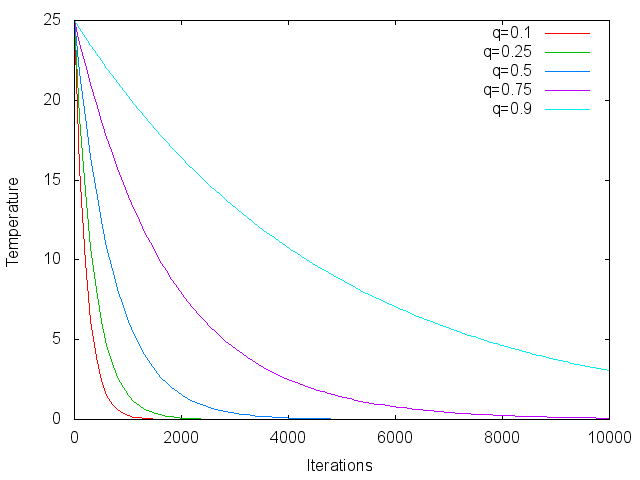
\includegraphics[scale=0.35]{./figures/temperature-drop}
  \caption{Temperature variations in standard SA with varying $q$}
  \label{fig:7}
\end{figure}
Figure~\ref{fig:7} shows how the temperature varies with iterations. It
clearly shows how the temperature drops quicker for smaller values of
$q$ and slower for larger values. Even though we removed the concept of
multiple number of mapping iterations per temperature level from the
previous algorithm, we retained the $q$ parameter as we wanted to
control how quickly or slowly the temperature must drop.

\item We use the value for the initial and final temperature for the
  annealing schedule from the paper written by Orsilla et
  al.~\cite{hors06}. Since the objective of this article is to map
  heterogeneous applications onto heterogeneous architectures, these
  heuristics have to be changed as well. We calculate the fastest and
  slowest processors by multiplying each processor's capabilities
  ($W^r_0(i) * W^r_1(i)$) and sorting them.

% \item The rest of the parameters remain the same as~\cite{hors06} and are subject to future work
% for changes if necessary.

\end{itemize} 

%%% Local Variables: 
%%% mode: latex
%%% TeX-master: "bare_conf"
%%% End: 


\section{EXPERIMENTS AND RESULTS}
\label{sec:exps}

\begin{table}[h!]
  \smaller{
  \centering
  \begin{tabular}{|c|c|c|c|c|c|c|}
    \hline
    \textbf{ } & 
    \multicolumn{6}{|c|}{\textbf{Applications}}\\
    \hline
    & Barcelona & Kyoto & San Francisco & Cologne & Lyon & Miami\\
    \hline
    $|V|$ & 13476 & 42456 & 15436 & 56548 & 8174 & 8141 \\
    \hline
    $|E|$ & 25658 & 93722 & 35092 & 115483 & 15586 & 21856 \\
    \hline
  \end{tabular}
  \caption{The task graph setup}
  }
  \label{tab:1}
\end{table}


\begin{figure*}[ht!]
  \centering
  \subfigure[Barcelona]{
    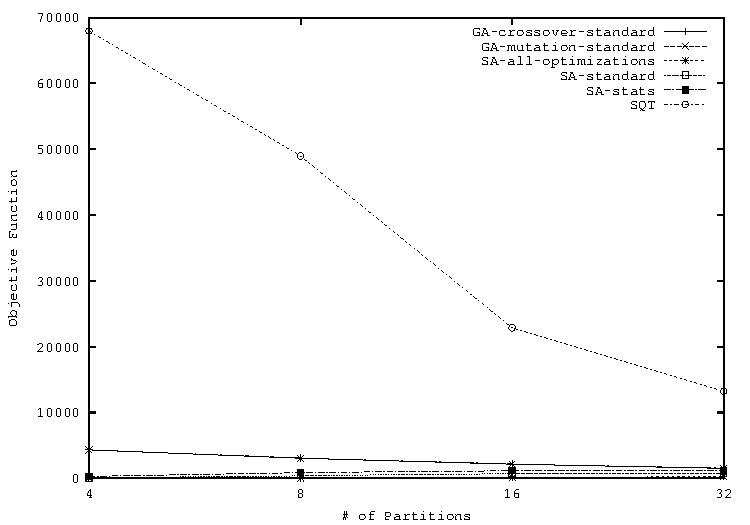
\includegraphics[angle=0, scale=0.4]{./figures/objective1/Barc.pdf}
    \label{fig:obj1barc}
  }
  \subfigure[Kyoto]{
    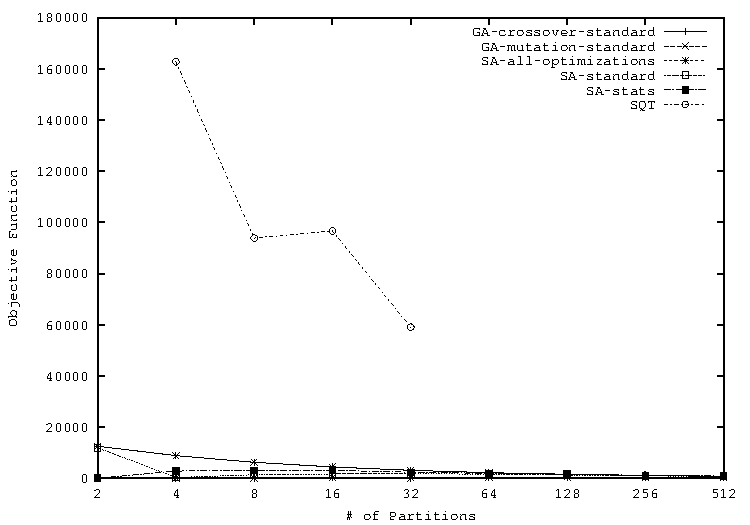
\includegraphics[angle=0, scale=0.4]{./figures/objective1/Kyoto}
    \label{fig:obj1kyoto}
  }
  \subfigure[San Francisco]{
    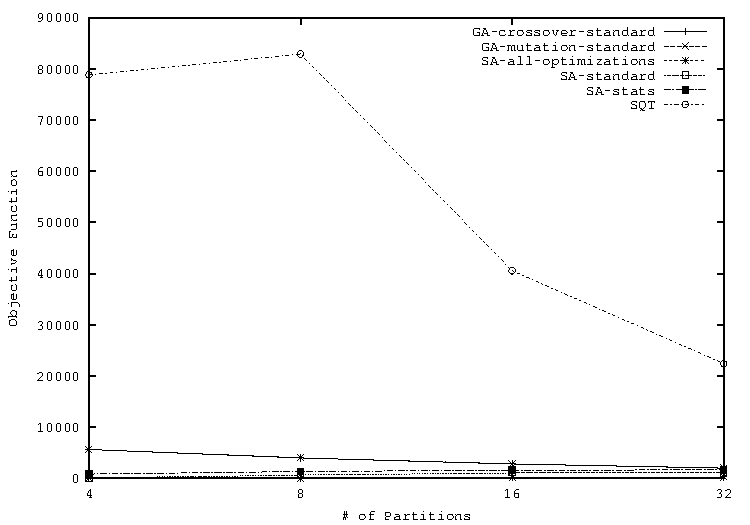
\includegraphics[angle=0, scale=0.4]{./figures/objective1/San}
    \label{fig:obj1san}
  }
  \subfigure[Cologne]{
    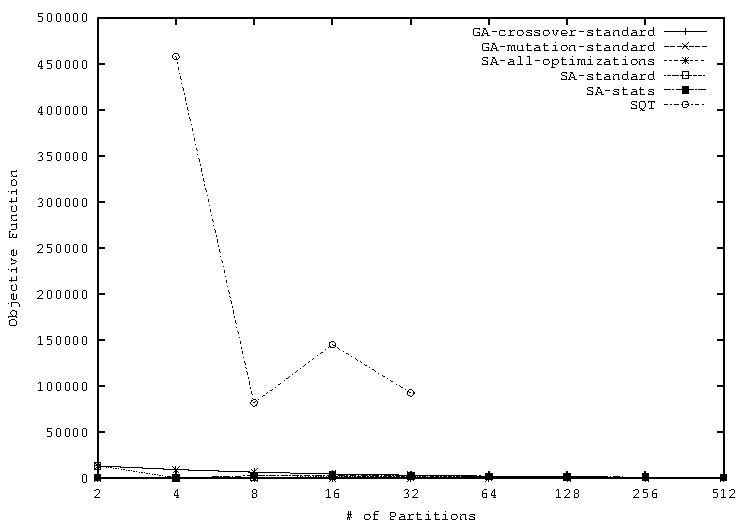
\includegraphics[angle=0, scale=0.4]{./figures/objective1/Cologne}
    \label{fig:obj1cologne}
  }
  \subfigure[Lyon]{
    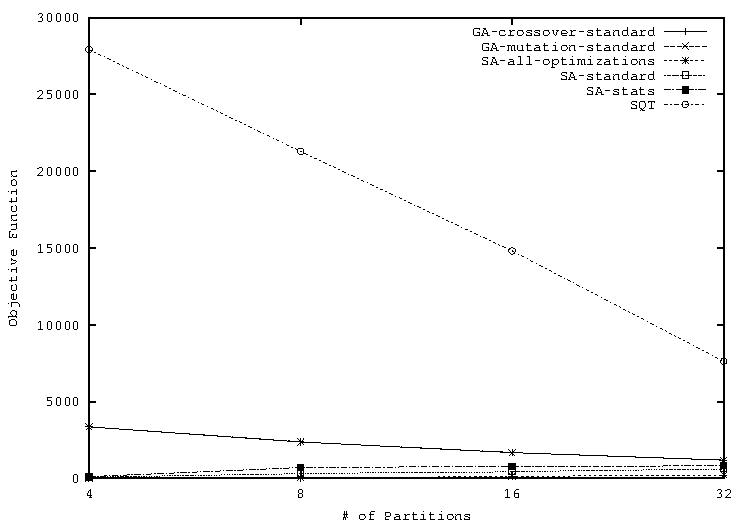
\includegraphics[angle=0, scale=0.4]{./figures/objective1/Lyon}
    \label{fig:obj1lyon}
  }
  \subfigure[Miami]{
    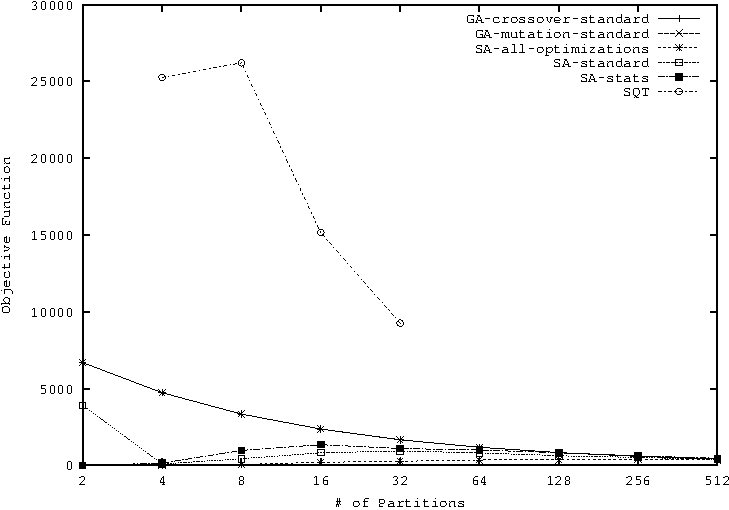
\includegraphics[angle=0, scale=0.4]{./figures/objective1/Miami}
    \label{fig:obj1miami}
  }
  \caption{Comparison of the partioning algorithms based on the first metric(Variance) given by Eq.~\ref{eq:metric3}}
  \label{fig:objective1}
\end{figure*}

\begin{figure*}[t!]
  \centering
  \subfigure[Barcelona]{
    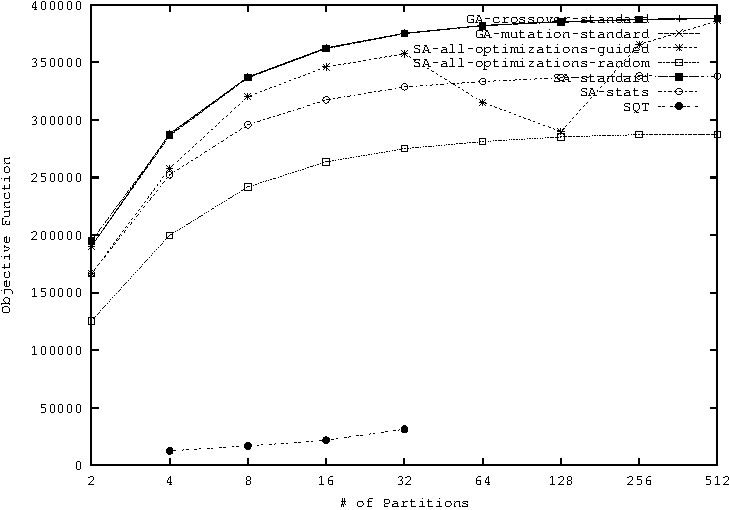
\includegraphics[angle=0, scale=0.4]{./figures/objective2/Barc}
    \label{fig:obj2barc}
  }
  \subfigure[Kyoto]{
    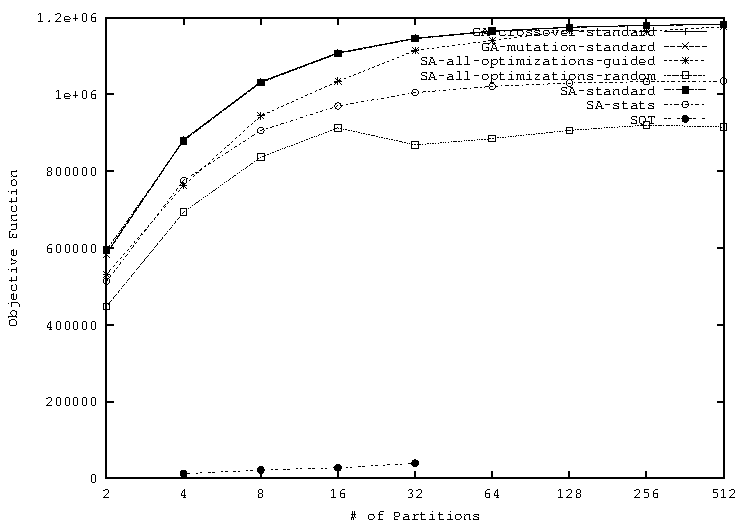
\includegraphics[angle=0, scale=0.4]{./figures/objective2/Kyoto}
    \label{fig:obj2kyoto}
  }
  \subfigure[San Francisco]{
    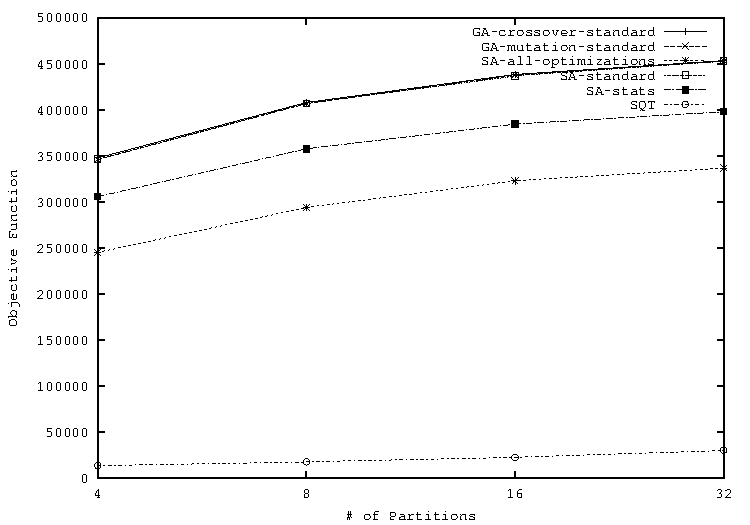
\includegraphics[angle=0, scale=0.4]{./figures/objective2/San}
    \label{fig:obj2san}
  }
  \subfigure[Cologne]{
    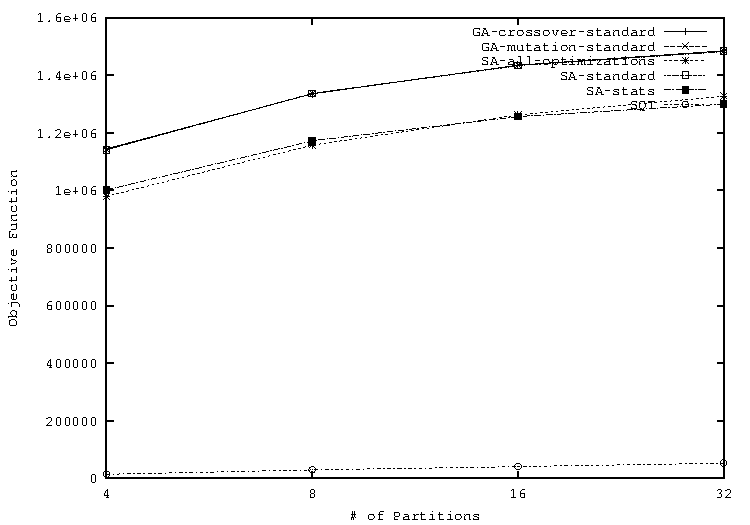
\includegraphics[angle=0, scale=0.4]{./figures/objective2/Cologne}
    \label{fig:obj2cologne}
  }
  \subfigure[Lyon]{
    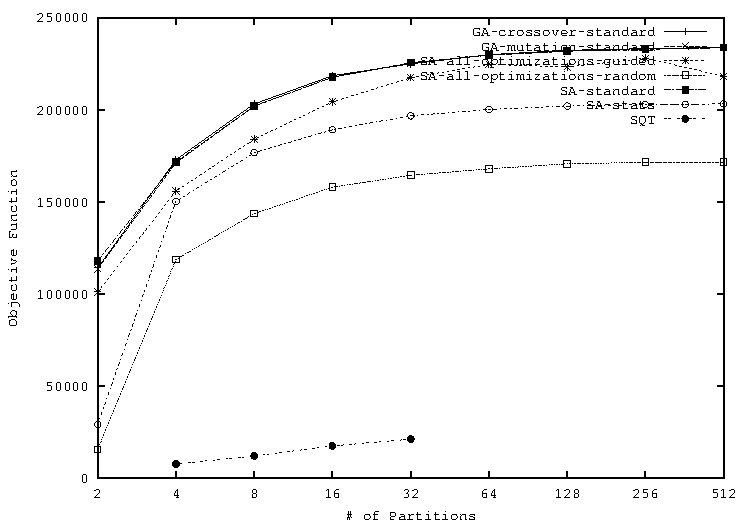
\includegraphics[angle=0, scale=0.4]{./figures/objective2/Lyon}
    \label{fig:obj2lyon}
  }
  \subfigure[Miami]{
    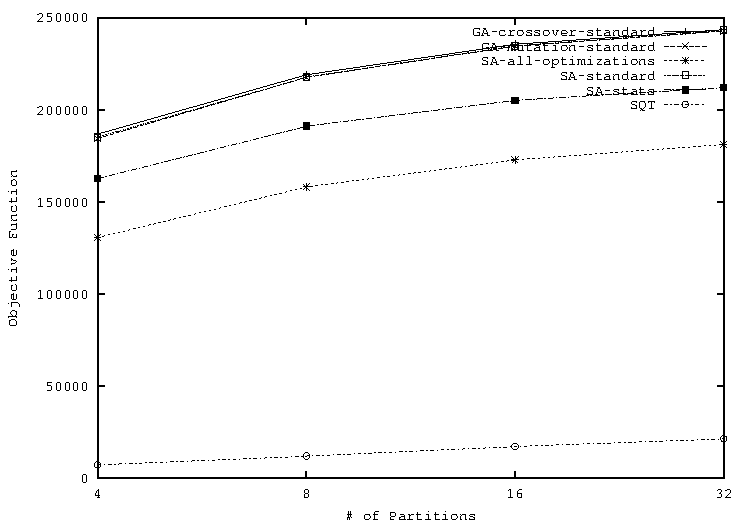
\includegraphics[angle=0, scale=0.4]{./figures/objective2/Miami}
    \label{fig:obj2miami}
  }
  \caption{Comparison of the partitioning algorithms based on the second metric(Inter-Partition Communication) given by Eq.~\ref{eq:metric2}}
  \label{fig:objective2}
\end{figure*}

\begin{figure*}[t!]
  \centering
  \subfigure[Barcelona]{
    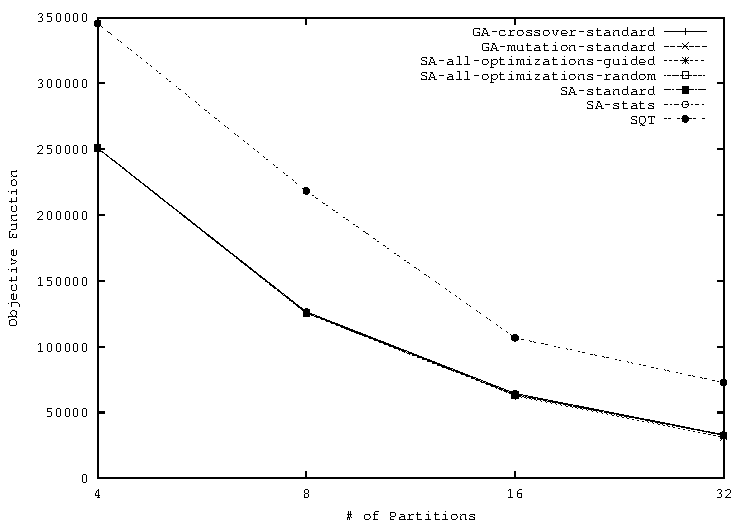
\includegraphics[angle=0, scale=0.4]{./figures/objective3/Barc}
    \label{fig:obj2barc}
  }
  \subfigure[Kyoto]{
    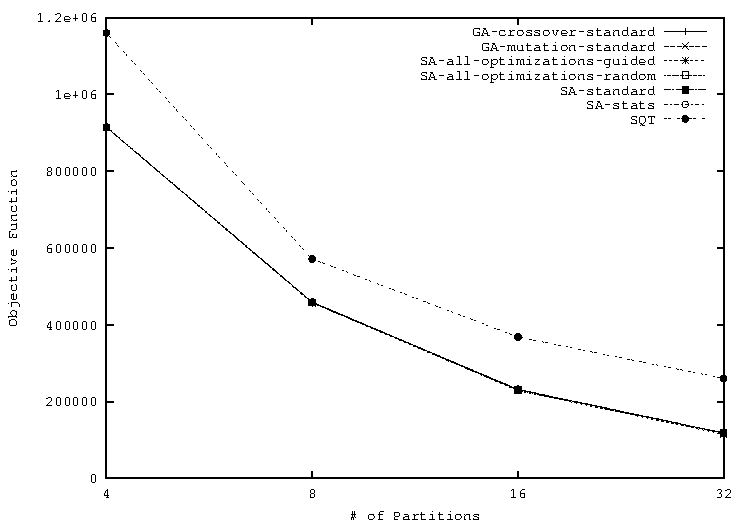
\includegraphics[angle=0, scale=0.4]{./figures/objective3/Kyoto}
    \label{fig:obj2kyoto}
  }
  \subfigure[San Francisco]{
    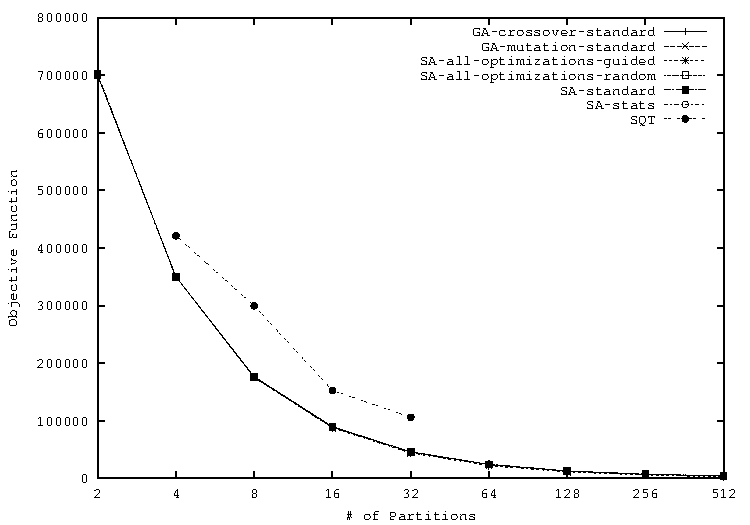
\includegraphics[angle=0, scale=0.4]{./figures/objective3/San}
    \label{fig:obj2san}
  }
  \subfigure[Cologne]{
    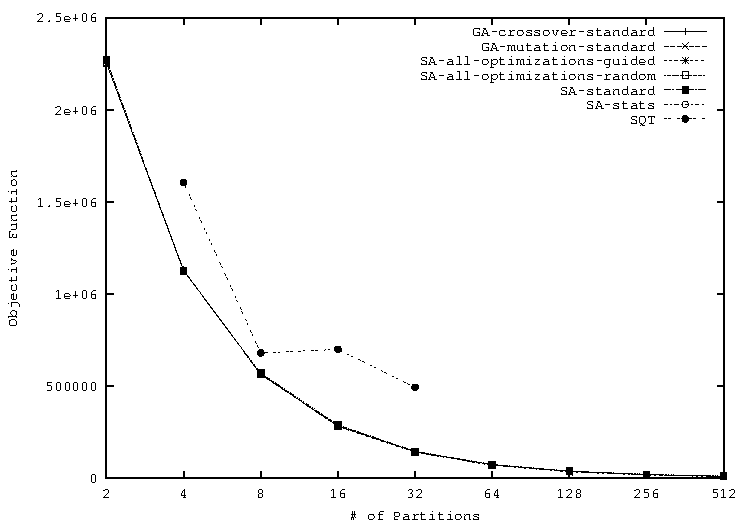
\includegraphics[angle=0, scale=0.4]{./figures/objective3/Cologne}
    \label{fig:obj2cologne}
  }
  \subfigure[Lyon]{
    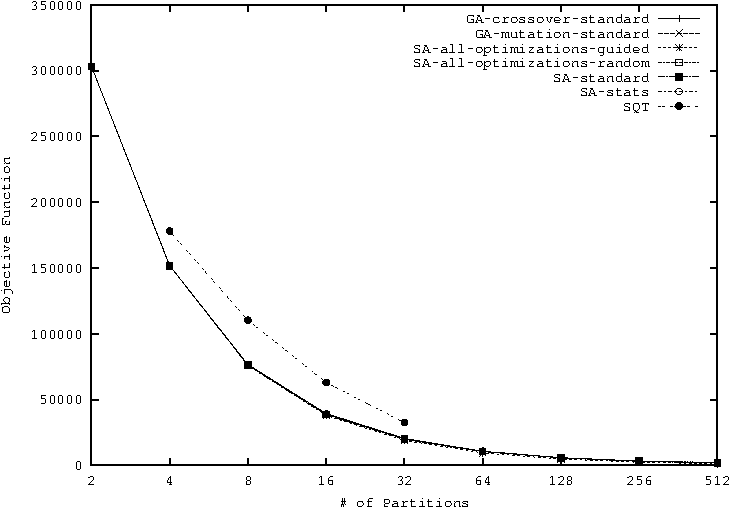
\includegraphics[angle=0, scale=0.4]{./figures/objective3/Lyon}
    \label{fig:obj2lyon}
  }
  \subfigure[Miami]{
    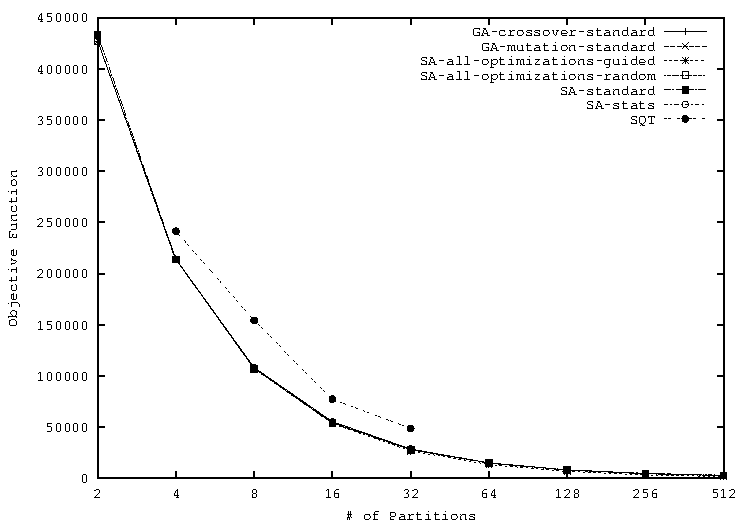
\includegraphics[angle=0, scale=0.4]{./figures/objective3/Miami}
    \label{fig:obj2miami}
  }
  \caption{Comparison of the partitioning algorithms based on the third metric(Max(PartitionSizes)) given by Eq.~\ref{eq:metric1}}
  \label{fig:objective2}
\end{figure*}

\section{FUTURE WORK}
\label{sec:futu}

\begin{itemize}
\item One of the limiting factors in this comparison is the limited representation of the road network. We plan to extend our model by allowing edges and vertices in our road network graph to have more than one weight associated with them. In doing so, we can allow for a finer and more accurate representation of the road network which in turn allows us to partition the graph better.
\item In the modified move function, we currently move edges(the neighbour correspoding to the edge) if it has a weight which is 2$\sigma$ away from $\mu$. This is under the assumption that traffic is normally distributed across the edges. One of the improvements that we could do is to fit the distribution of traffic across edges and move edges according to this regressively found curve that fits the traffic distribution.
\end{itemize}

\section{Conclusion}
\label{sec:conclusion}

In this paper we have outlined the comparison of space and graph partitioning techniques in the context of partitioning road network graphs for simulation. We have discussed 

\section*{Acknowledgement}
This work is partly funded by the IRCSET Enterprise Partnership Scheme in
collaboration with IBM Research, Ireland.


% The authors would like to thank...
% more thanks here

\scriptsize{
\bibliographystyle{ieeetran}
% \bibliography{latex8}
\bibliography{bare_conf}
}


% that's all folks
\end{document}